\chapter{Umsetzung der interaktiven Benutzeroberfläche}
\label{chapter:umsetzung-der-interaktiven-benutzeroberfläche}

TODO:

{\color{white}
\begin{myverbbox}{\patchworkCLI}
The board game Patchwork implemented in Rust with different AI players. Type "help" for more information.
> console
Player 1: Human(name: Anonymer Modelleisenbahnliebhaber)
Player 2: Greedy
────────────────────────────────────────────────── TURN 1 ───────────────────────────────────────────────────
Current player is 1
...
────────────────────────────────────────────────── TURN 13 ──────────────────────────────────────────────────
Current player is 1
Player (button balance: 10): │ Player (button balance: 1):
  ▓▓▓█████▓⬜  │   ▓▓▓▓▓▓▓▓▓
  ███████▓▓⬜  │   ▓▓▓▓▓▓███
  █▓▓██▓▓▓▓⬜  │   ▓▓▓▓████▓
  ▓▓▓▓█▓▓▓▓⬜  │   ▓▓██████▓
  ▓▓▓▓▓▓▓▓▓⬜  │   ▓▓███████
  ▓▓▓▓▓▓▓▓▓⬜  │   ▓▓██████▓
  ▓▓▓▓▓▓▓▓▓⬜  │   ▓▓▓█▓▓█▓▓
  ▓▓▓▓▓▓▓▓▓⬜  │   ▓▓▓▓▓▓▓▓▓
  ▓▓▓▓▓▓▓▓▓⬜  │   ▓▓▓▓▓▓▓▓▓
      Button income: 0       │      Button income: 3
Time board:
┌─┬─┬─┬─┬─┬─┬─┬─┬─┬─┬─┬─┬─┬─┬─┬─┬─┬─┬─┬─┬─┬─┬─┬─┬─┬─┬─┬─┬─┬─┬─┬─┬─┬─┬─┬─┬─┬─┬─┬─┬─┬─┬─┬─┬─┬─┬─┬─┬─┬─┬─┬─┬─┬─┐
│ │ │ │ │ │B│ │ │ │ │ │B│ │ │ │1│2│B│ │ │ │ │ │B│ │ │P│ │ │B│ │ │P│ │ │B│ │ │P│ │ │B│ │ │P│ │ │B│ │ │P│ │ │B│
└─┴─┴─┴─┴─┴─┴─┴─┴─┴─┴─┴─┴─┴─┴─┴─┴─┴─┴─┴─┴─┴─┴─┴─┴─┴─┴─┴─┴─┴─┴─┴─┴─┴─┴─┴─┴─┴─┴─┴─┴─┴─┴─┴─┴─┴─┴─┴─┴─┴─┴─┴─┴─┴─┘
Next 6 patches (can only take first 3):
⬜█⬜⬜        ⬜⬜⬜⬜        ⬜⬜⬜⬜        █⬜⬜⬜        ██
⬜█⬜⬜        ⬜⬜⬜⬜        ⬜⬜⬜⬜        █⬜⬜⬜        ██
⬜█⬜⬜        █⬜⬜⬜        ██⬜⬜        ██⬜⬜        ⬜█⬜⬜         ⬜█
███⬜        ███⬜        ██⬜⬜        █⬜⬜⬜        ⬜█⬜⬜         ██
Id: 12            Id: 19            Id: 9             Id: 10            Id: 13             Id: 21
Income: 2         Income: 1         Income: 2         Income: 1         Income: 3          Income: 0
Button cost: 7    Button cost: 4    Button cost: 6    Button cost: 2    Button cost: 10    Button cost: 1
Time cost: 2      Time cost: 2      Time cost: 5      Time cost: 3      Time cost: 5       Time cost: 3
'Anonymer Modelleisenbahnliebhaber' can choose one of the actions: 'take 1', 'take 2', 'take 3', 'walk'.
> Please enter the action: take 2
You chose to place the following patch:
   █⬜⬜   Id: 19       Button cost: 4
   ███   Income: 1    Time cost: 2
> Please enter the  rotation (0, 90, 180, 270) and orientation (if flipped: y/n) of the patch: 0,n
> Please enter the row and column of the patch (row, column): 5,5
Player 'HumanPlayer(name: Anonymer Modelleisenbahnliebhaber)' chose action:
Action 402 - Patch(12) placement (index 0) at (4, 4) with (R 0°, O normal) (P12I0═4‖4↻0↔0P1) after 15.95s
\end{myverbbox}
}

\definecolor{maximizeWindowColor}{HTML}{f5df09}
\definecolor{minimizeWindowColor}{HTML}{56bd73}
\definecolor{closeWindowColor}{HTML}{ea4f44X}

\begin{figure}[!ht]
    \centering
    \resizebox{\textwidth}{!}{\begin{tikzpicture}
            \node [text=white,inner sep=0pt,,outer sep=0pt,clip,rounded corners=0.15cm] (cli) at (0,0) {\sffamily \patchworkCLI};
            \node[circle,fill=closeWindowColor, minimum size = 0.15cm, above right = 0.3cm and -0.3cm of cli] (close) {};
            \node[circle,fill=maximizeWindowColor, minimum size = 0.15cm, left = 0.15cm of close] (maximize) {};
            \node[circle, fill=minimizeWindowColor, minimum size = 0.15cm, left = 0.15cm of maximize] {};
            \node[text=white] at ($ (cli.north) + (0,0.45) $) {\sffamily \textbf{Patchwork 1.0.0 (Release Build) | Fabian Wolf \& Nico Zeitz}} ;
            \begin{pgfonlayer}{back}
                \filldraw[fill=black,draw=black,rounded corners=0.15cm] ($ (cli.north west) + (-0.25,0.85) $) rectangle ($ (cli.south east) + (0.25,-0.25) $);
            \end{pgfonlayer}
            \begin{pgfonlayer}{shadow}
                \shade[outercolor,inner color=innercolor,outer color=outercolor] ($(cli.south west)+(-0.25,0.25)+(\shadowshift)+(\shadowradius/2,\shadowradius/2)$) circle (\shadowradius);
                \shade[outercolor,inner color=innercolor,outer color=outercolor] ($(cli.north west)+(-0.25,0.85)+(\shadowshift)+(\shadowradius/2,-\shadowradius/2)$) circle (\shadowradius);
                \shade[outercolor,inner color=innercolor,outer color=outercolor] ($(cli.south east)+(0.25,0.25)+(\shadowshift)+(-\shadowradius/2,\shadowradius/2)$) circle (\shadowradius);
                \shade[outercolor,inner color=innercolor,outer color=outercolor] ($(cli.north east)+(0.25,0.85)+(\shadowshift)+(-\shadowradius/2,-\shadowradius/2)$) circle (\shadowradius);
                \shade[top color=innercolor,bottom color=outercolor] ($(cli.south west)+(-0.25,0.25)+(\shadowshift)+(\shadowradius/2,-\shadowradius/2)$) rectangle ($(cli.south east)+(0.25,0.25)+(\shadowshift)+(-\shadowradius/2,\shadowradius/2)$);
                \shade[left color=innercolor,right color=outercolor] ($(cli.south east)+(0.25,0.25)+(\shadowshift)+(-\shadowradius/2,\shadowradius/2)$) rectangle ($(cli.north east)+(0.25,0.85)+(\shadowshift)+(\shadowradius/2,-\shadowradius/2)$);
                \shade[bottom color=innercolor,top color=outercolor] ($(cli.north west)+(-0.25,0.85)+(\shadowshift)+(\shadowradius/2,-\shadowradius/2)$) rectangle ($(cli.north east)+(0.25,0.85)+(\shadowshift)+(-\shadowradius/2,\shadowradius/2)$);
                \shade[outercolor,right color=innercolor,left color=outercolor] ($(cli.south west)+(-0.25,0.25)+(\shadowshift)+(-\shadowradius/2,\shadowradius/2)$) rectangle ($(cli.north west)+(-0.25,0.85)+(\shadowshift)+(\shadowradius/2,-\shadowradius/2)$);
                \filldraw ($(cli.south west)+(-0.25,0.25)+(\shadowshift)+(\shadowradius/2,\shadowradius/2)$) rectangle ($(cli.north east)+(0.25,0.85)+(\shadowshift)-(\shadowradius/2,\shadowradius/2)$);
            \end{pgfonlayer}
        \end{tikzpicture}}
    \caption[CLI Schnittstelle des Patchwork Spiels]{\acs{CLI} Schnittstelle des Patchwork Spiels}
    \label{fig:patchwork-console-ui}
\end{figure}

TODO:

\begin{figure}[!ht]
    \centering
    \resizebox{\textwidth}{!}{\begin{tikzpicture}
        \node [inner sep=0pt,,outer sep=0pt,clip,rounded corners=0.15cm] (image) at (0,0) {
            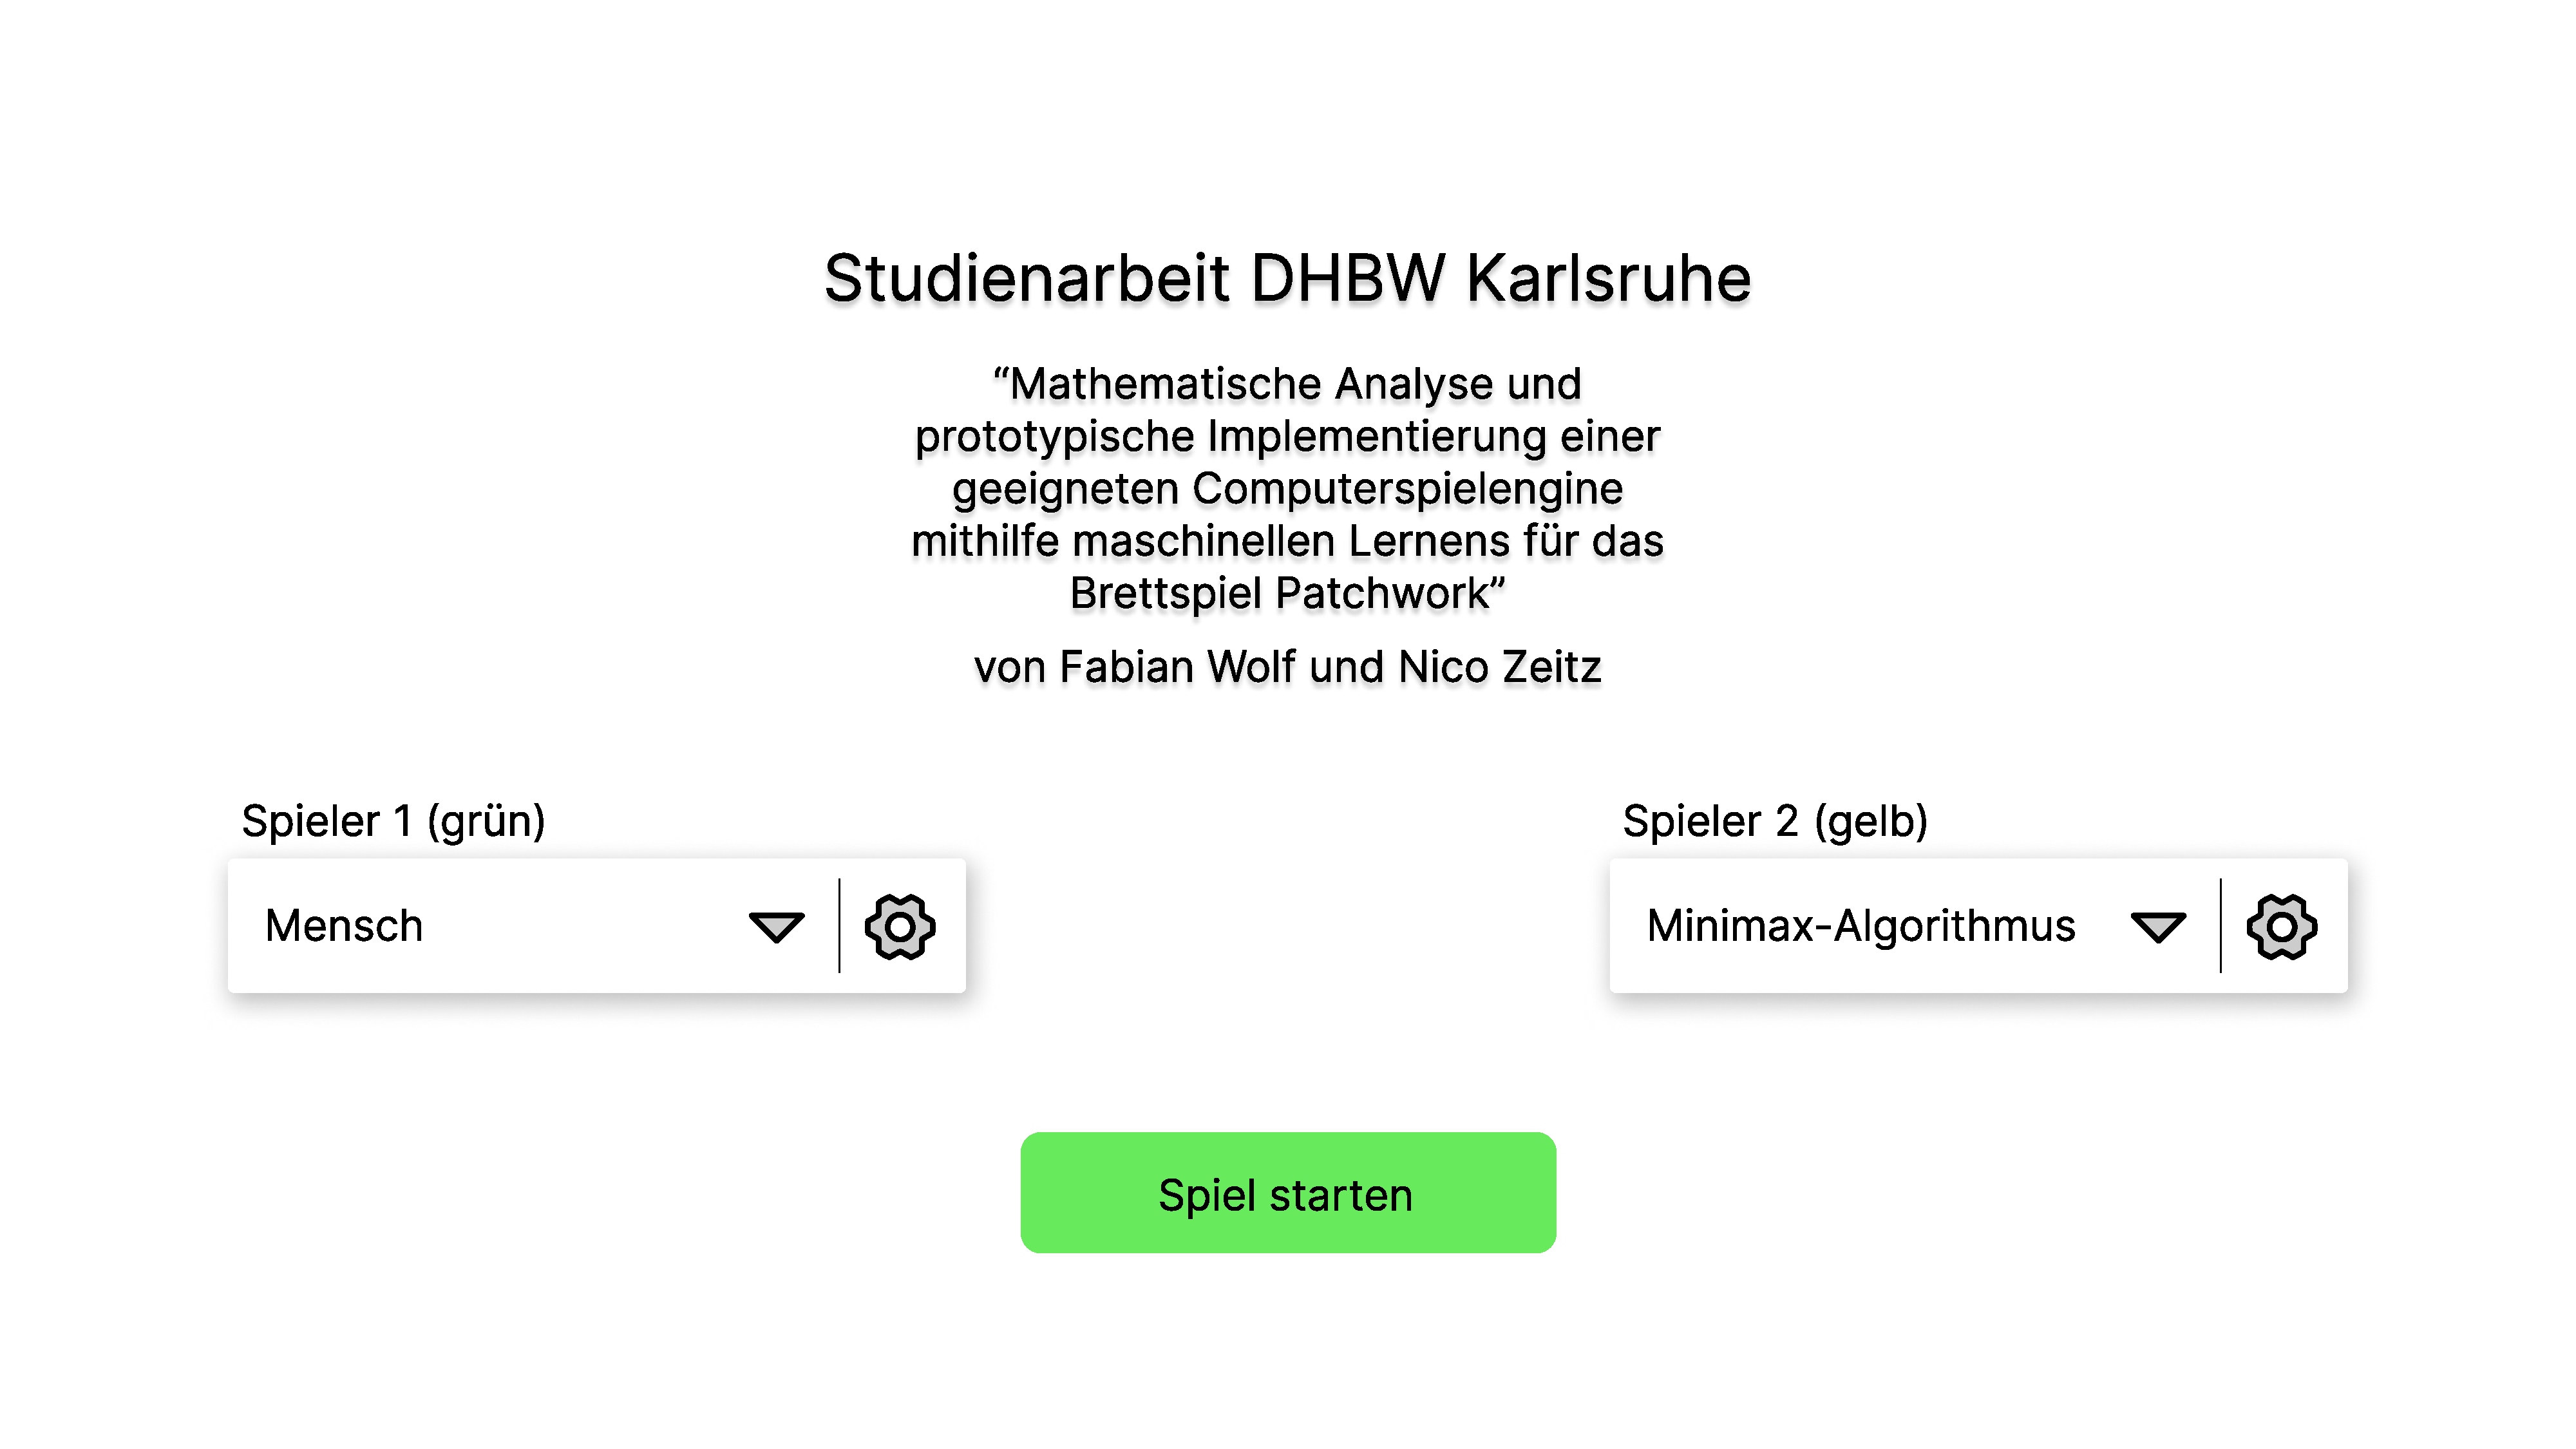
\includegraphics[width=\textwidth]{res/pictures/desig_main_ui.pdf}};
        \drawshadow{image}
    \end{tikzpicture}}
    \caption{Designentwurf vom Hauptmenü des Computerspiel}
    \label{fig:design-main-ui}
\end{figure}

\begin{figure}[!ht]
    \centering
    \resizebox{\textwidth}{!}{\begin{tikzpicture}
        \node [inner sep=0pt,,outer sep=0pt,clip,rounded corners=0.15cm] (image) at (0,0) {
            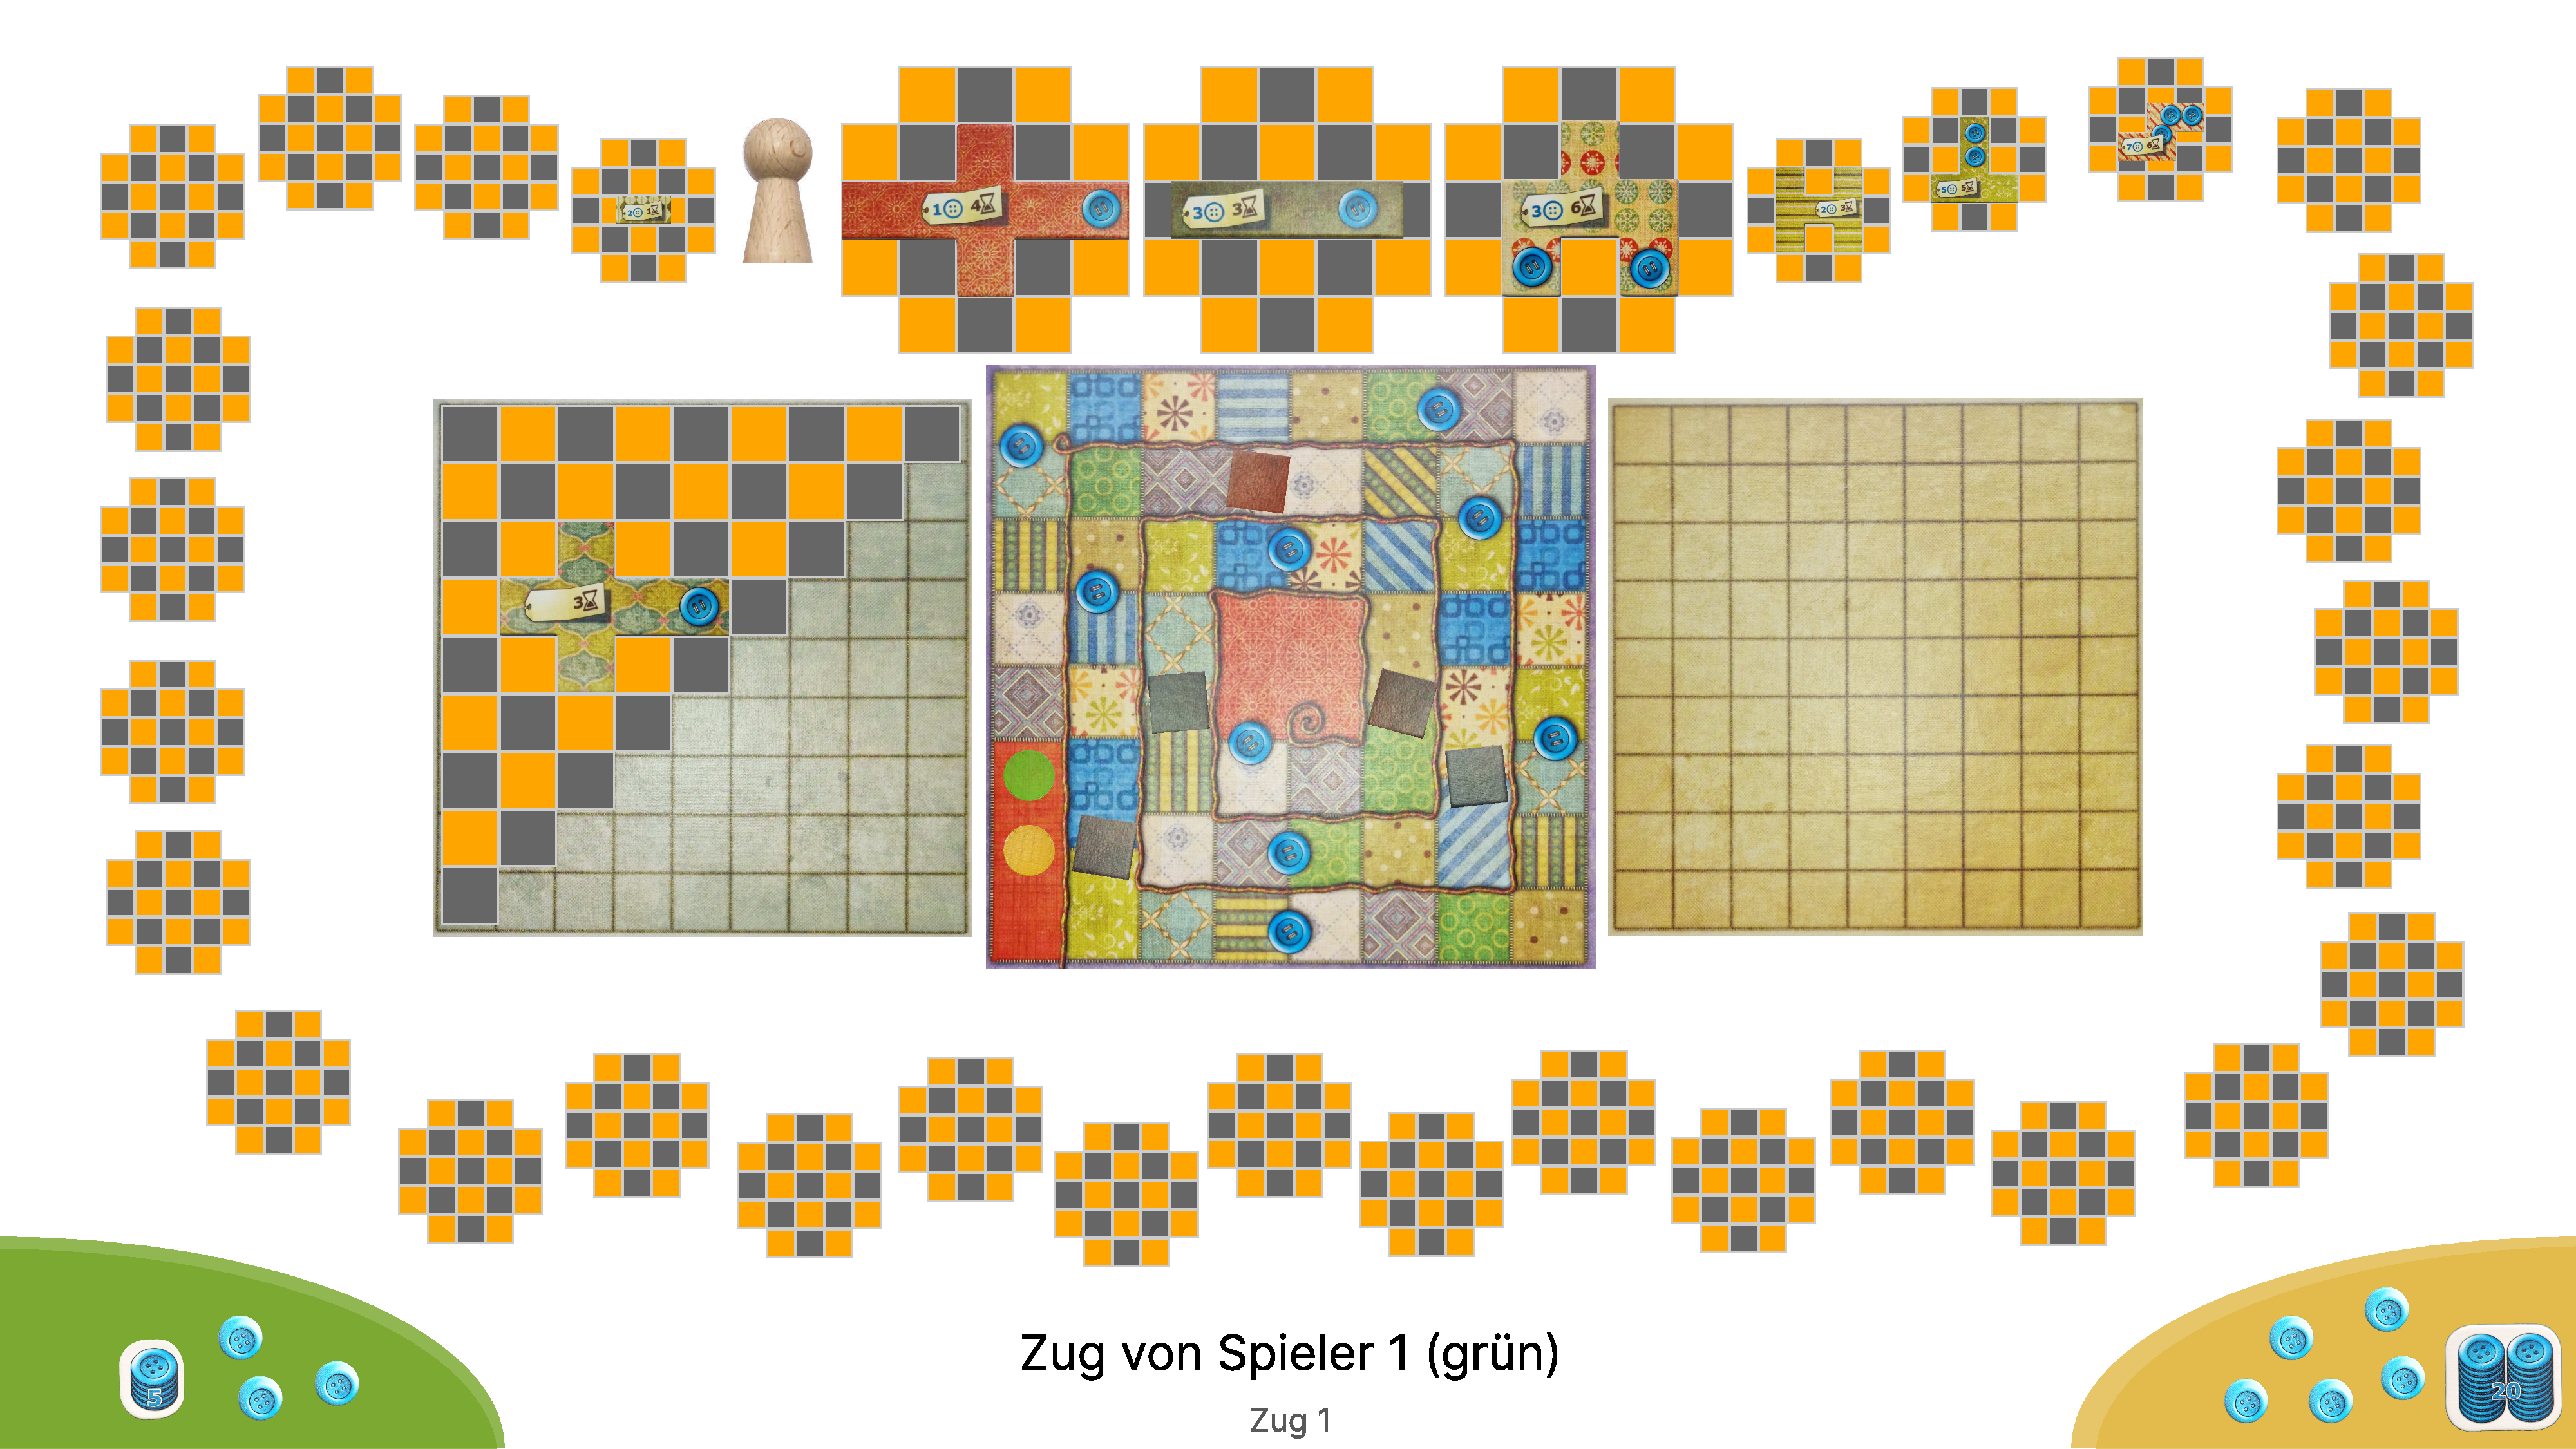
\includegraphics[width=\textwidth]{res/pictures/design_game_ui.pdf}};
        \drawshadow{image}
    \end{tikzpicture}}
    \caption{Designentwurf der grafische Benutzeroberfläche des Computerspiel}
    \label{fig:design-game-ui}
\end{figure}



\begin{figure}[!ht]
    \centering
    \resizebox{\textwidth}{!}{\begin{tikzpicture}
        \node [inner sep=0pt,,outer sep=0pt,clip,rounded corners=0.15cm] (image) at (0,0) {
            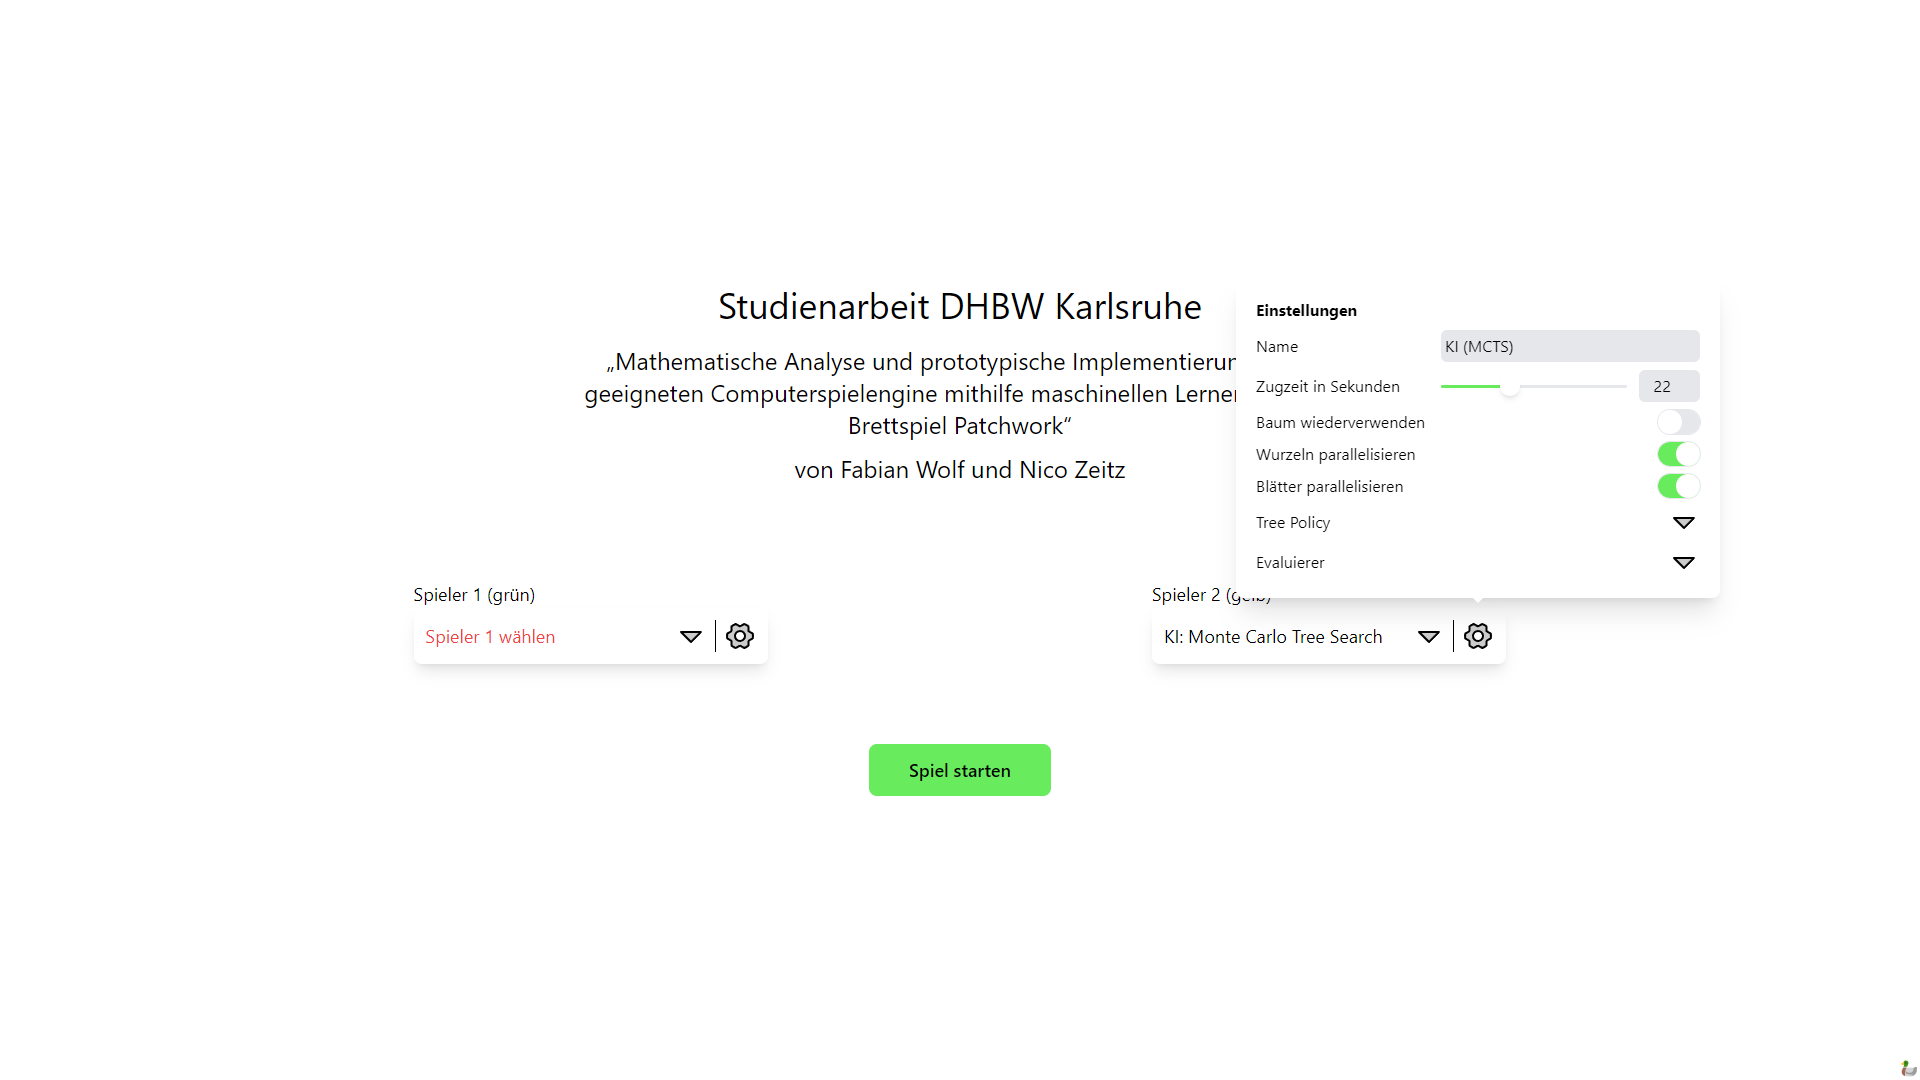
\includegraphics[width=\textwidth]{res/pictures/final_main_ui.png}};
        \drawshadow{image}
    \end{tikzpicture}}
    \caption{Umsetzung des Hauptmenü des Computerspiel}
    \label{fig:final-main-ui}
\end{figure}



\begin{figure}[!ht]
    \centering
    \resizebox{\textwidth}{!}{\begin{tikzpicture}
        \node [inner sep=0pt,,outer sep=0pt,clip,rounded corners=0.15cm] (image) at (0,0) {
            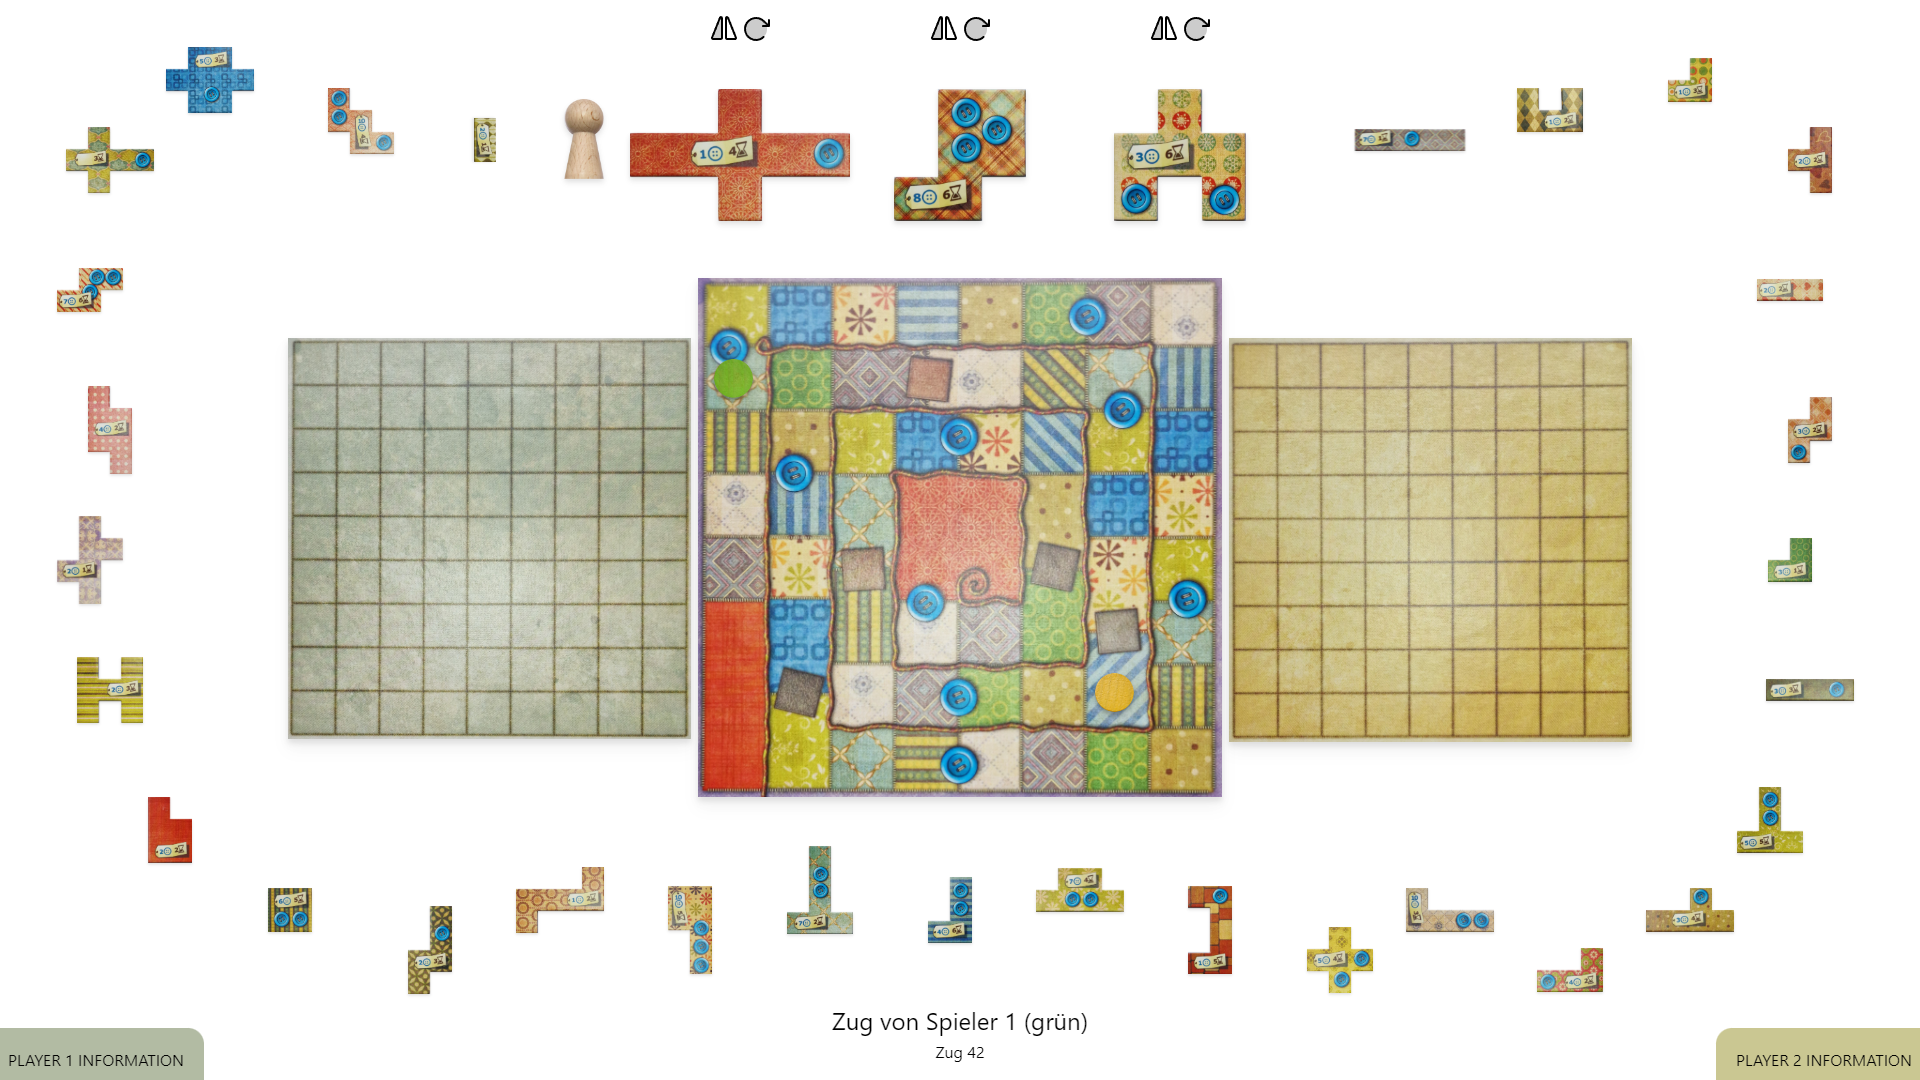
\includegraphics[width=\textwidth]{res/pictures/final_game_ui.png}};
        \drawshadow{image}
    \end{tikzpicture}}
    \caption{Umsetzung der grafische Benutzeroberfläche des Computerspiel}
    \label{fig:final-game-ui}
\end{figure}